%!TeX program = xelatex
\documentclass[12pt,hyperref,a4paper,UTF8]{ctexart}
\usepackage{zjureport}
\usepackage{listings}
\usepackage{enumitem}
\usepackage{float}
\usepackage{xcolor}
\usepackage{amsmath}
\lstset{
    %backgroundcolor=\color{red!50!green!50!blue!50},%代码块背景色为浅灰色
    basicstyle=\footnotesize\ttfamily,
    rulesepcolor= \color{gray}, %代码块边框颜色
    breaklines=true,  %代码过长则换行
    numbers=left, %行号在左侧显示
    numberstyle= \small,%行号字体
    keywordstyle= \color{blue},%关键字颜色
    commentstyle=\color{gray}, %注释颜色
    frame=shadowbox%用方框框住代码块
    }


%%-------------------------------正文开始---------------------------%%
\begin{document}

%%-----------------------封面--------------------%%
\cover

%%------------------摘要-------------%%
%\begin{abstract}
%
%在此填写摘要内容
%
%\end{abstract}

\thispagestyle{empty} % 首页不显示页码

%%--------------------------目录页------------------------%%
\newpage
\tableofcontents

%%------------------------正文页从这里开始-------------------%
\newpage

%%可选择这里也放一个标题
%\begin{center}
%    \title{ \Huge \textbf{{标题}}}
%\end{center}
\section{选题背景}

在语音识别技术迅速发展的今天，语音识别系统已广泛应用于各个领域，包括语音助手、智能家居、自动客服等。尤其是连续数字串的语音识别在银行账户验证、电话号码输入和智能控制等方面具有重要应用价值。然而，如何有效地提取语音信号的特征并进行准确的识别仍然是一个具有挑战性的问题。

在人工智能课程中，我们系统地学习了机器学习的基础理论和应用方法，包括隐马尔可夫模型（HMM）、深度神经网络（DNN）等模型，并深入了解了这些模型在语音识别领域的实际应用。语音识别作为人工智能的重要研究方向之一，具有广泛的应用场景，例如语音助手、智能家居和自动客服等。

基于课程的学习，我们决定将语音识别作为课程项目的研究方向。

在连续数字串的语音识别系统设计中，主要面临以下几个关键问题：

1. \textbf{语音特征提取：} 语音信号具有非平稳性和复杂性，需要通过有效的特征提取方法将其转换为具有代表性的特征参数。梅尔频率倒谱系数（MFCC）是一种常用且有效的语音特征提取方法，能够较好地反映语音信号的频谱特征。

2. \textbf{语音活动检测（VAD）：} 在连续语音信号中，需要准确地分离出语音段和非语音段。VAD算法能够帮助系统有效地检测和分割语音信号，从而提高后续识别过程的效率和准确性。

3. \textbf{机器学习模型的选择与训练：} 选择合适的机器学习算法，并对模型进行训练，以实现高效的语音识别。常用的模型包括隐马尔可夫模型（HMM）、深度神经网络（DNN）和卷积神经网络（CNN）等。这些模型需要大量的语音数据进行训练，以提高识别的准确率。

4. \textbf{连续数字串的识别：} 在实际应用中，语音信号通常是连续的，包含多个数字串。如何在连续语音信号中准确地识别和分割每个数字，是实现高性能语音识别系统的一个难点。

基于以上问题，本设计提出了一种基于MFCC特征、
VAD算法和机器学习的连续数字串语音识别系统设计方案。
该方案旨在通过有效的特征提取、准确的语音活动检测和高效的机器学习模型，
实现对连续数字串语音信号的准确识别。本文将详细介绍系统的设计思路、关键技术和实现方法，
并对实验结果进行分析和讨论。

\begin{figure}[H]
    \centering
    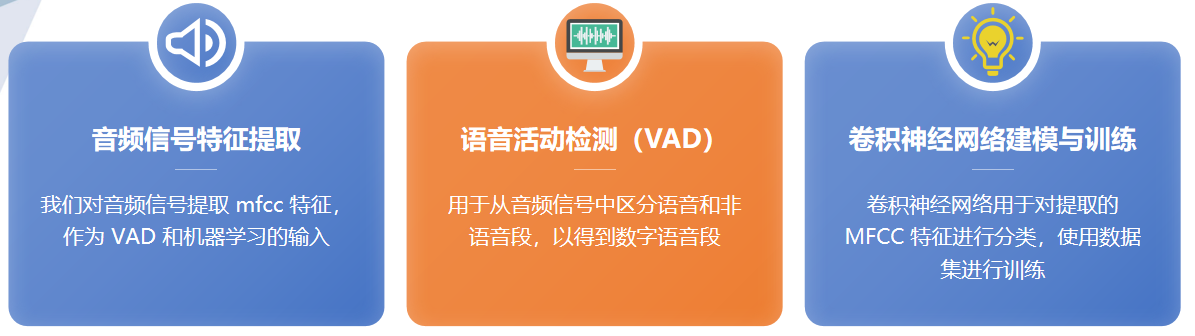
\includegraphics[width=0.8\linewidth]{./figures/fig/image7.png}
    \caption{连续数字语音识别系统设计}
    \label{fig:flowchart}
\end{figure}


\section{MFCC特征提取}

梅尔频率倒谱系数（Mel Frequency Cepstral Coefficients，简称MFCC）是语音信号处理中广泛应用的一种特征提取方法。它通过模拟人类听觉系统的感知方式，对语音信号进行分析和处理，从而获取更能反映语音本质特征的参数。
以下简单介绍MFCC和实现MFCC特征提取过程。具体的代码实现可以参考仿照代码中的mfcc文件夹中的内容。

\subsection{MFCC简介}

\subsection*{梅尔刻度（Mel Scale）}
人耳对频率的感知是ff线性的，低频部分的分辨率较高，而高频部分的分辨率较低。梅尔刻度正是用来模拟这种非线性的感知方式。将实际频率转换为梅尔刻度的公式如下：

\begin{equation*}
    Mel = 2595 \times \log_{10}(1 + \frac{Frequency}{700})
\end{equation*}
从梅尔刻度转换回实际频率的公式为：
\begin{equation*}
    Frequency = 700 \times (10^{\frac{Mel}{2595}} - 1)
\end{equation*}



梅尔刻度的引入，使得频率的变化更符合人耳的听觉特性，有效地模拟了听觉系统对声音的处理过程。

\subsection*{临界带（Critical Band）和mel滤波器}
人耳对声音的感知不仅与频率有关，还与频率的分布密切相关。临界带将频率划分为若干个频带，每个频带对应一个滤波器。这些滤波器的集合被称为Mel滤波器组（Mel filter bank）。研究表明，人耳对200Hz到5kHz范围内的语音信号最为敏感，这一频段对语音的清晰度有重要影响。

当两个不同响度的声音同时存在时，响度较大的声音会掩蔽响度较小的声音，这种现象被称为掩蔽效应。低频声音在内耳蜗基底膜上的行波传递距离大于高频声音，因此低频声音更容易掩蔽高频声音。基于这一特性，Mel滤波器组设计为从低频到高频按临界带宽的大小由密到疏排列，对输入信号进行带通滤波。每个滤波器输出的信号能量作为基本特征，进一步处理后可作为语音识别的输入特征。
\newpage

\subsection{MFCC算法实现}

在本项目中，我们实现了梅尔频率倒谱系数（MFCC）特征提取算法，具体步骤如下：

\begin{enumerate}
    \item \textbf{预加重（Pre-emphasis）}：通过高通滤波器增强语音信号的高频部分，补偿高频成分的衰减。
    \item \textbf{分帧（Framing）}：将语音信号分割为短时帧，每帧通常为20-40毫秒，并设置一定的帧移以保证帧间重叠。
    \item \textbf{加窗（Windowing）}：对每帧信号乘以汉明窗，减少帧边界的不连续性。
    \item \textbf{短时傅里叶变换（STFT）}：对每帧信号进行快速傅里叶变换（FFT），计算频谱幅值和功率谱。
    \item \textbf{Mel滤波器组（Mel Filter Bank）}：构建Mel滤波器组，将功率谱映射到Mel频率域。
    \item \textbf{对数变换（Logarithm）}：对Mel频谱取对数，模拟人耳对声音强度的感知。
    \item \textbf{离散余弦变换（DCT）}：对对数Mel频谱进行离散余弦变换，提取MFCC系数。
    \item \textbf{正弦提升器（Liftering）}：对MFCC系数应用正弦提升器，改善频谱质量。
\end{enumerate}

\begin{figure}[H]
    \centering
    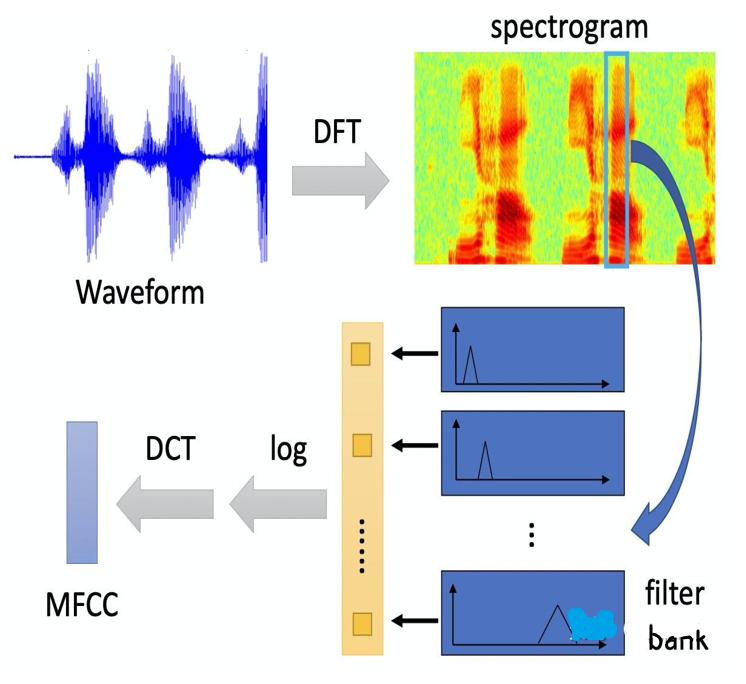
\includegraphics[width=0.65\linewidth]{./figures/fig/image8.png}
    \caption{MFCC特征提取流程}
    \label{fig:flowchart}
\end{figure}

以下是MFCC特征提取的部分关键实现步骤（完整代码请参考项目代码文件中的mfcc/mfcc.ipynb与mfcc.py）：

\begin{lstlisting}[language=Python, caption=MFCC算法关键代码]
# 预加重
pre_emphasis = 0.97
signal_preemphasized = np.append(signal[0], signal[1:] - pre_emphasis * signal[:-1])

# 分帧和加窗
frame_length = int(0.025 * sample_rate)
frame_step = int(0.01 * sample_rate)
frames = np.array([signal_preemphasized[i:i+frame_length] * np.hamming(frame_length)
                   for i in range(0, len(signal_preemphasized) - frame_length, frame_step)])

# FFT和功率谱
NFFT = 512
mag_frames = np.absolute(np.fft.rfft(frames, NFFT))
pow_frames = (1.0 / NFFT) * (mag_frames ** 2)

# Mel滤波器组
mel_filters = mel_filter_bank(num_filters=40, NFFT=NFFT, sample_rate=sample_rate)
mel_spectrogram = np.dot(pow_frames, mel_filters.T)

# 对数变换和DCT
log_mel_spectrogram = np.log(mel_spectrogram + 1e-10)
mfcc = dct(log_mel_spectrogram, type=2, axis=1, norm='ortho')[:, 1:13]
\end{lstlisting}

通过上述实现，我们成功提取了语音信号的MFCC特征，并与Librosa库的实现进行了对比，验证了算法的正确性。以下是MFCC特征的可视化结果：

\newpage

\section{语音活动检测(VAD)}
语音活动检测（Voice Activity Detection，简称VAD）是一种用于识别语音信号中的语音片段和非语音片段的技术。其主要目的是在连续的音频信号中区分出哪些部分是包含语音活动的，从而过滤掉背景噪声和静音部分，提高后续处理的效率和准确性。

VAD算法广泛应用于各种语音处理系统中，包括语音识别、语音增强、语音编码和语音合成等。通过准确地检测出语音活动段，可以减少处理不必要的无用信息，从而提高系统的性能和可靠性。

\subsection{VAD算法简介}
VAD算法有多种实现方法，每种方法都有其优缺点和适用场景。以下是几种常见的VAD算法实现方法：

\begin{enumerate}
    \item \textbf{基于能量的VAD}：通过计算音频信号的短时能量来判断是否存在语音活动。此方法计算简单，但在低信噪比环境下表现较差。
    \item \textbf{基于谱熵的VAD}：通过计算音频信号每帧频谱的熵值来判断语音活动。该方法对包含大量噪声的音频信号有较好的鲁棒性，但计算复杂度相对较高。
    \item \textbf{基于自相关函数的VAD}：利用信号的自相关特性来区分语音和噪声。该方法能有效地区分语音信号和噪声信号，但对非稳态噪声的处理效果有限。
    \item \textbf{基于机器学习的VAD}：通过训练分类器（如支持向量机、神经网络等）来识别语音活动。该方法具有较高的准确性和鲁棒性，但依赖于大量的训练数据和较高的计算资源。
    \item \textbf{基于深度学习的VAD}：利用卷积神经网络（CNN）、长短时记忆网络（LSTM）等深度学习模型，捕捉更复杂的特征和语音活动模式。该方法在复杂噪声环境和多种语言的语音信号处理中表现出色，但同样需要大量的训练数据和高性能计算资源。
\end{enumerate}

\subsection{基于mfcc特征提取和无监督机器学习的VAD算法实现}
本设计使用基于mfcc特征提取和无监督机器学习（如K-means聚类）的VAD算法。其是一种结合了语音信号分析和机器学习技术的方法。该算法首先使用MFCC特征提取算法提取出语音信号的特征向量，然后使用无监督机器学习算法（如K-means聚类）对特征向量进行聚类分析，将包含语音活动的特征向量划分为一个聚类，将包含非语音活动的特征向量划分为另一个聚类。最后，根据聚类结果判断当前帧是否包含语音活动。


\begin{figure}[H]
    \centering
    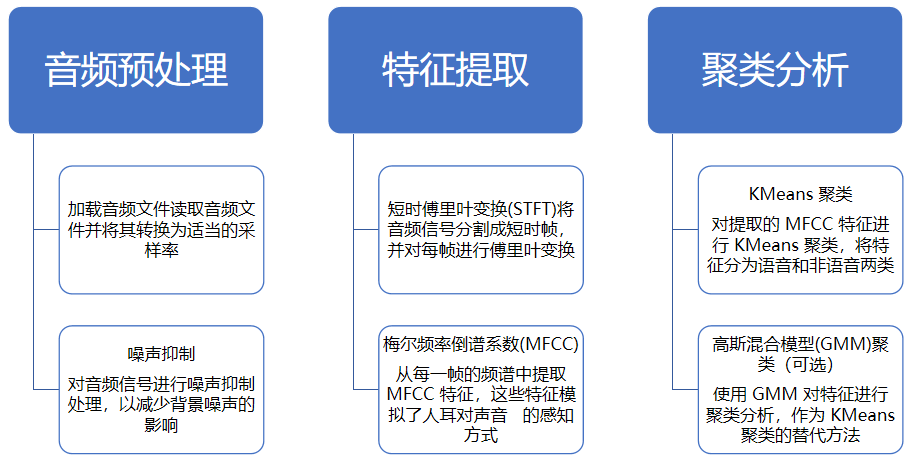
\includegraphics[width=0.85\linewidth]{./figures/fig/image9.png}
    \caption{VAD算法流程图}
    \label{fig:flowchart}
\end{figure}

算法大致实现步骤如下：\textbf{完整代码实现参考源码vad文件夹下的py程序}

\subsection*{音频预处理}

首先，我们加载音频文件并对其进行预处理，包括采样率调整和噪声抑制。

\begin{lstlisting}[language=Python, caption=加载音频文件并进行噪声抑制]
def load_audio(file_path, sr=8000):
    # 使用librosa读取音频
    audio, sr = librosa.load(file_path, sr=sr)
    # 应用噪声抑制
    audio = nr.reduce_noise(y=audio, sr=sr)
    return audio, sr
\end{lstlisting}

在此步骤中，我们使用了 \texttt{librosa} 库加载音频，并通过 \texttt{noisereduce} 库对音频进行噪声抑制，以减少背景噪声的影响。

\subsection*{特征提取}

接下来，我们从音频信号中提取MFCC特征，这些特征能够有效地表征音频信号的频谱特性。

\begin{lstlisting}[language=Python, caption=提取MFCC特征]
def extract_mfcc(audio, sr):
    mfccs = librosa.feature.mfcc(y=audio, sr=sr, n_mfcc=NUM_MFCC)
    return mfccs.T  # 转置矩阵，使得每行对应一个时间段
\end{lstlisting}

在此步骤中，我们使用 \texttt{librosa.feature.mfcc} 函数提取了音频的MFCC特征，并将其转置以便后续处理。

\subsection*{聚类分析}

我们使用KMeans算法对提取的MFCC特征进行聚类，将音频信号分为语音段和非语音段两类。


\begin{lstlisting}[language=Python, caption=KMeans聚类]
def perform_clustering(features):
    kmeans = KMeans(n_clusters=NUM_CLUSTERS)
    labels = kmeans.fit_predict(features)
    return labels
\end{lstlisting}

在此步骤中，我们将MFCC特征输入到KMeans聚类模型中，并获得每一帧的聚类标签。

\subsection*{语音段检测}

根据聚类标签，我们计算每个聚类的平均能量，并通过能量大小判断哪个聚类代表“无声”。
然后，我们根据标签变化检测语音段的起始和结束位置。

\begin{lstlisting}[language=Python, caption=语音段检测]
def get_voiced_segments(audio, labels):
    voiced_segments = []
    energy_0 = np.mean([np.sum(audio[i*HOP_SIZE:(i+1)*HOP_SIZE]**2) for i in range(len(labels)) if labels[i] == 0])
    energy_1 = np.mean([np.sum(audio[i*HOP_SIZE:(i+1)*HOP_SIZE]**2) for i in range(len(labels)) if labels[i] == 1])
    silence_label = 0 if energy_0 < energy_1 else 1

    start_idx = None
    for i in range(1, len(labels)):
        if labels[i] != labels[i-1]:
            if labels[i-1] == silence_label:
                start_idx = i * HOP_SIZE
            elif start_idx is not None:
                end_idx = i * HOP_SIZE
                voiced_segments.append((start_idx, end_idx))
                start_idx = None
    if start_idx is not None:
        end_idx = len(audio)
        voiced_segments.append((start_idx, end_idx))
    return voiced_segments
\end{lstlisting}

\subsection*{后处理}

为了避免将相邻的语音段误认为多个独立段，我们对检测到的语音段进行合并。

\begin{lstlisting}[language=Python, caption=合并相邻语音段]
def merge_close_segments(voiced_segments, threshold=1024):
    merged_segments = []
    start_idx, end_idx = voiced_segments[0]
    for next_start_idx, next_end_idx in voiced_segments[1:]:
        if next_start_idx - end_idx <= threshold:
            end_idx = next_end_idx
        else:
            merged_segments.append((start_idx, end_idx))
            start_idx, end_idx = next_start_idx, next_end_idx
    merged_segments.append((start_idx, end_idx))
    return merged_segments
\end{lstlisting}

\subsection*{结果保存与评估}

最后，我们将检测到的语音段保存到文本文件中，并使用评估函数计算F1分数、
准确率、召回率和精确率。

\begin{lstlisting}[language=Python, caption=评估VAD算法性能]
def evaluate(data_length, label_input, predict_input):
    ...
    accuracy = acc / data_length
    recall = tp / voice_length
    precision = tp / predict_voice_length
    f1_score = (2 * precision * recall) / (precision + recall)
    return f1_score, accuracy, recall, precision
\end{lstlisting}

\newpage

\section{语音识别（ASR）}

\subsection{语音识别简介}

语音识别（Automatic Speech Recognition，简称ASR）是指将人类的语音信号转换为相应的文本或指令的技术。随着计算机科学和人工智能的发展，语音识别技术在过去几十年里取得了显著进展，并在各个领域得到了广泛应用，如智能助手（如Siri、Google Assistant）、语音翻译、语音控制的设备和应用（如智能家居、汽车语音控制系统）等。

语音识别的工作流程一般包括以下几个步骤：
\begin{enumerate}
    \item \textbf{语音信号预处理}：对采集到的语音信号进行降噪、预加重、分帧、加窗等处理，以提高信号的质量和后续特征提取的效果。
    \item \textbf{特征提取}：从预处理后的语音信号中提取出能够有效表征语音内容的特征参数，如梅尔频率倒谱系数（MFCC）、线性预测倒谱系数（LPCC）等。
    \item \textbf{声学模型}：使用统计模型（如高斯混合模型，GMM）或深度学习模型（如卷积神经网络，CNN，或长短时记忆网络，LSTM）将提取的特征参数映射到音素或音素序列。
    \item \textbf{语言模型}：根据语言的结构和统计规律，对识别出的音素序列进行解码，生成最有可能的词或句子。
    \item \textbf{后处理}：对识别结果进行修正和优化，如纠错、标点符号添加等，以提高识别文本的准确性和可读性。
\end{enumerate}

\subsection*{语音识别的实现}
语音识别技术有多种实现方法，以下是几种常见的方法及其特点：

\begin{enumerate}
    \item \textbf{基于模板匹配的方法}：这种方法将待识别的语音信号与预先存储的模板进行比较，以找到最匹配的模板。主要包括动态时间规整（Dynamic Time Warping，DTW）方法。此方法适用于小词汇量的应用，但对大词汇量和复杂语音信号的识别效果较差。
    
    \item \textbf{基于隐马尔可夫模型（HMM）的方法}：隐马尔可夫模型是语音识别领域中最早广泛应用的统计模型。HMM可以有效地处理语音信号的时序性和变异性，通过训练得到的HMM模型可以用于识别语音信号中的音素序列。该方法对中小型词汇量的语音识别有较好的效果。
    
    \item \textbf{基于神经网络的方法}：随着深度学习的发展，基于神经网络的方法在语音识别中得到了广泛应用。主要包括卷积神经网络（CNN）、递归神经网络（RNN）、长短时记忆网络（LSTM）等。这些模型能够捕捉语音信号中的复杂特征和时序关系，大大提高了语音识别的准确率。特别是端到端（End-to-End）的深度学习模型，可以直接将语音信号映射到文本序列，简化了传统语音识别的复杂流程。
    
    \item \textbf{基于Transformer的方法}：近年来，Transformer模型在自然语言处理领域取得了突破性的进展，也被引入到语音识别中。基于Transformer的模型，如Transformers和其变体（如BERT、GPT-3），可以处理长距离的依赖关系和上下文信息，进一步提高了语音识别的效果。
    
    \item \textbf{混合模型的方法}：将不同模型的优势结合起来，如HMM-DNN（深度神经网络与隐马尔可夫模型结合）方法，利用HMM处理时序信息，DNN处理非线性特征。这种方法在大型语音识别系统中得到了成功应用。
\end{enumerate}



\subsection{基于卷积神经网络（CNN）的语音识别算法实现}

我们的语音识别系统采用基于卷积神经网络（CNN）的语音识别系统的实现。
该算法主要包括数据预处理、特征提取、模型构建、训练和推理等步骤。
以下是对每个步骤的具体描述。具体的完整代码实现参考源代码。


\subsection*{数据预处理与特征提取}

训练使用的数据集来源于网络开源语音数据。
音频数据通过 \texttt{scipy.io.wavfile} 库读取，
并使用 \texttt{python\_speech\_features} 库提取 MFCC 特征。
特征提取包括计算一阶和二阶差分特征，并对特征矩阵进行截取或填充以统一形状。


\begin{lstlisting}[language=Python, caption=MFCC特征提取]
def get_mfcc(data, fs):
    wav_feature = mfcc(data, fs, numcep=6)
    feature = wav_feature.reshape(1, -1, 6)
    if feature.shape[1] > 64:
        feature = feature[:, :64, :]
    else:
        feature = np.pad(feature, ((0, 0), (0, 64-feature.shape[1]), (0, 0)), 'constant')
    feature = feature.transpose((2, 0, 1))
    return feature
\end{lstlisting}

特征提取后的数据被组织为数据集，并通过 \texttt{DataLoader} 
加载以供模型训练和推理使用。

\subsection*{模型构建}

我们设计了一个卷积神经网络（CNN）模型，包含多个卷积层、批归一化层、
激活函数、全连接层和 Dropout 层。以下是模型的参数：

\begin{lstlisting}[language=Python, caption=CNN模型结构]
// filepath: c:\Users\Huang Xianmin\Desktop\人工智能\finalpro\code\asr\Model.py
class Audio(nn.Module):
    def __init__(self):
        super(Audio, self).__init__()
        self.conv1 = nn.Conv2d(6, 32, 1, 1, 1)
        self.bn1 = nn.BatchNorm2d(32)
        self.conv2 = nn.Conv2d(32, 32, (3, 2), (1, 2), (1, 0))
        self.bn2 = nn.BatchNorm2d(32)
        self.conv3 = nn.Conv2d(32, 64, 3, 1, 1)
        self.bn3 = nn.BatchNorm2d(64)
        self.conv4 = nn.Conv2d(64, 64, (3, 2), (1, 2), (1, 0))
        self.bn4 = nn.BatchNorm2d(64)
        self.conv5 = nn.Conv2d(64, 128, 3, 1, 1)
        self.bn5 = nn.BatchNorm2d(128)
        self.conv6 = nn.Conv2d(128, 128, (3, 2), 2)
        self.bn6 = nn.BatchNorm2d(128)
        self.fc1 = nn.Linear(8*128, 256)
        self.dropout = nn.Dropout(0.5)
        self.fc2 = nn.Linear(256, 10)

    def forward(self, inputs, labels=None):
        out = F.relu(self.bn1(self.conv1(inputs)))
        out = F.relu(self.bn2(self.conv2(out)))
        out = F.relu(self.bn3(self.conv3(out)))
        out = F.relu(self.bn4(self.conv4(out)))
        out = F.relu(self.bn5(self.conv5(out)))
        out = F.relu(self.bn6(self.conv6(out)))
        out = out.view(out.size(0), -1)
        out = F.relu(self.fc1(out))
        out = self.dropout(out)
        out = self.fc2(out)
        return out
\end{lstlisting}

\subsection*{模型训练}

模型训练使用 AdamW 优化器和交叉熵损失函数，并结合学习率调度器和 L2 正
则化以提高模型性能。

\begin{lstlisting}[language=Python, caption=模型训练]
def train_model(model, train_loader, dev_loader, epochs=20):
    optimizer = optim.AdamW(model.parameters(), lr=0.001, weight_decay=0.001)
    scheduler = optim.lr_scheduler.ReduceLROnPlateau(optimizer, 'max', patience=3, factor=0.1)
    criterion = nn.CrossEntropyLoss()

    for epoch in range(epochs):
        model.train()
        for features, labels in train_loader:
            features = features.float().to('cuda' if torch.cuda.is_available() else 'cpu')
            labels = labels.to('cuda' if torch.cuda.is_available() else 'cpu')
            outputs = model(features)
            loss = criterion(outputs, labels)
            optimizer.zero_grad()
            loss.backward()
            optimizer.step()
\end{lstlisting}

\subsection*{模型推理}

推理阶段加载训练好的模型权重，并对测试数据进行预测。

\begin{lstlisting}[language=Python, caption=模型推理]
def infer_model(model, test_loader):
    model.eval()
    with torch.no_grad():
        for features, labels in test_loader:
            features = features.float().to('cuda' if torch.cuda.is_available() else 'cpu')
            outputs = model(features)
            _, predicted = torch.max(outputs.data, 1)
            print(f"Predicted labels: {predicted}")
\end{lstlisting}

\subsection*{模型效果}

通过上述实现，我们在测试集上评估了模型的性能，测试集的准确率达到了 90\% 以上。
模型训练和测试得到的结果如下：

\begin{figure}[H]
    \centering
    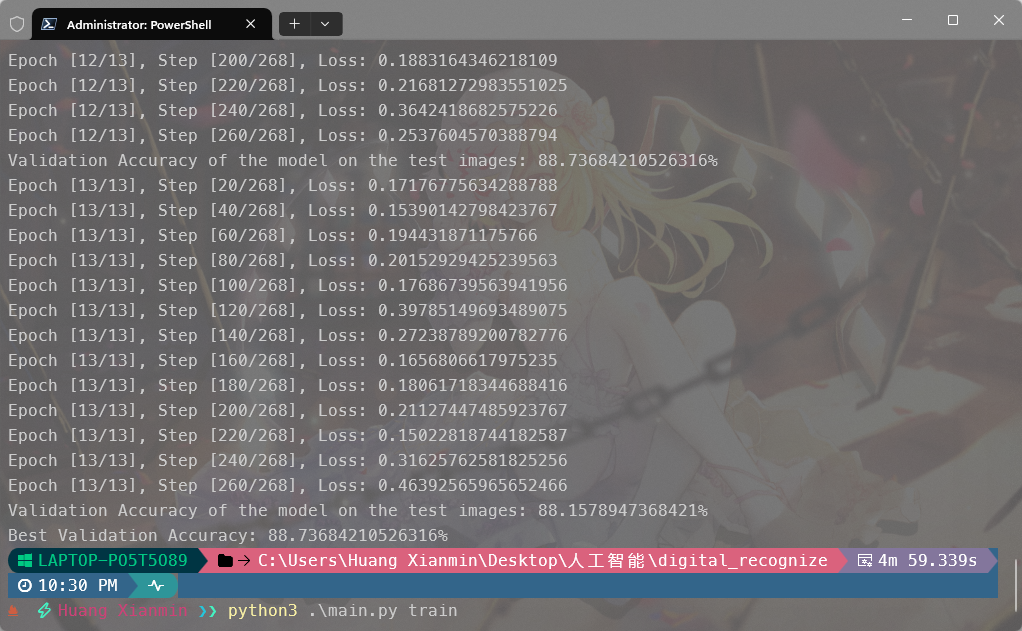
\includegraphics[width=0.88\linewidth]{./figures/fig/image6.png}
    \caption{模型训练过程}
\end{figure}

\begin{figure}[H]
    \centering
    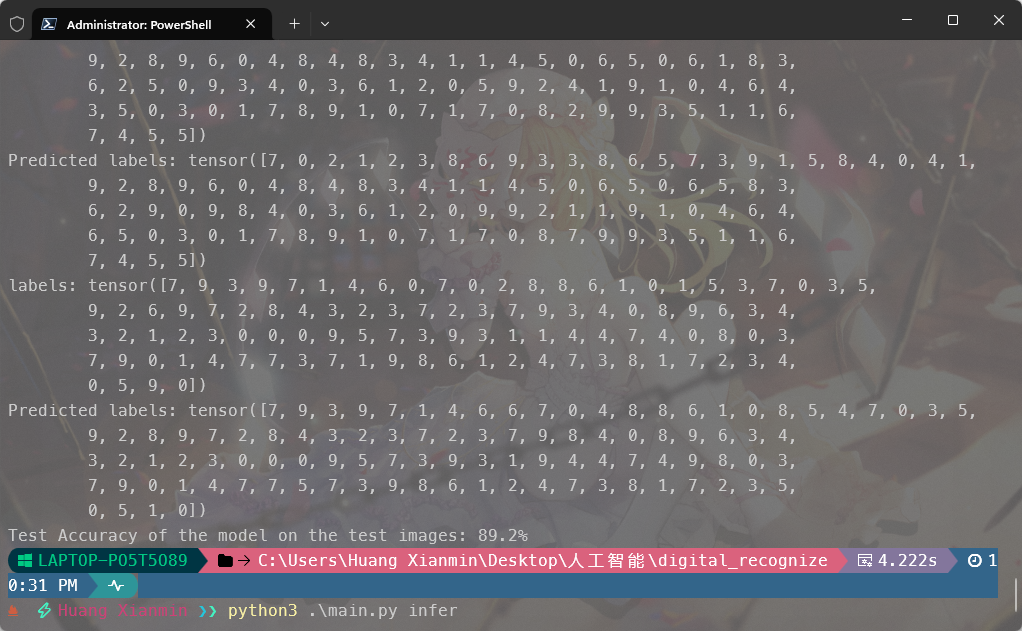
\includegraphics[width=0.88\linewidth]{./figures/fig/image5.png}
    \caption{模型测试效果}
\end{figure}

由于程序仅为课程设计的实现，
使用模型的复杂度较低，训练用数据集较小，
因此模型效果可能无法达到实际应用的要求。但是，通过训练和测试，
模型在测试集上的准确率基本能达到了90\%以上。

此外，模型的性能和泛化能力仍有不足，对于差异性较大的音频样本，
模型可能无法准确识别，此外也可能存在一些过拟合的现象。
因此，在实际应用中，需要进一步优化模型结构和参数，
并使用更多的数据集进行训练和测试。



\newpage

\section{连续数字语音识别系统}

结合前面的MFCC特征提取、VAD算法和CNN模型，我们实现了一个连续数字语音识别系统。
系统的主要功能是对输入的连续数字语音信号进行分段、特征提取和分类，从而实现对数字语音的准确识别。以下是系统的框架和架构的详细介绍。

\subsection{系统框架}

系统的整体架构可以分为以下几个模块：
\begin{enumerate}
    \item \textbf{音频信号特征提取}：从输入的音频信号中提取MFCC特征，作为后续VAD和CNN模型的输入。
    \item \textbf{语音活动检测（VAD）}：通过VAD算法将音频信号分割为语音段和非语音段，提取出包含数字语音的有效片段。
    \item \textbf{卷积神经网络建模与训练}：设计并训练一个CNN模型，用于对提取的MFCC特征进行分类，识别出每段语音对应的数字。
    \item \textbf{输入信号识别}：结合VAD和CNN模型，对输入的连续数字语音信号进行分段和分类，最终输出识别结果。
    \item \textbf{图形用户界面（GUI）}：提供一个用户友好的界面，支持音频文件选择、播放、录音、绘制时域图和频域图、执行VAD分段以及语音识别等功能。
\end{enumerate}

\subsection{系统实现}

\subsection*{音频信号特征提取}

音频信号的特征提取使用了MFCC算法。通过 \texttt{python\_speech\_features} 库提取MFCC特征，并对特征矩阵进行截取或填充以统一形状。提取的MFCC特征作为后续VAD和CNN模型的输入。

\subsection*{语音活动检测（VAD）}

VAD模块通过 \texttt{webrtcvad} 库实现，能够将音频信号分割为语音段和非语音段。VAD的主要功能是过滤掉静音和背景噪声，仅保留包含语音活动的片段，从而提高后续识别的效率和准确性。

\subsection*{卷积神经网络建模与训练}

CNN模型是系统的核心部分，用于对提取的MFCC特征进行分类。模型的结构包括多个卷积层、批归一化层、激活函数、全连接层和Dropout层。模型的训练使用了AdamW优化器和交叉熵损失函数，并结合学习率调度器和L2正则化以提高模型性能。

\subsection*{输入信号识别}

系统对输入的音频信号进行以下处理：
\begin{enumerate}
    \item 使用VAD算法将输入音频分为多个语音段，每个段落对应一个数字语音。
    \item 对每段音频提取MFCC特征。
    \item 将每段音频的MFCC特征输入CNN模型进行推理，得到对应的数字识别结果。
\end{enumerate}

\subsection*{图形用户界面（GUI）}

系统提供了一个基于Tkinter的图形用户界面，支持以下功能：
\begin{itemize}
    \item 选择音频文件并播放。
    \item 录制音频并保存为WAV文件。
    \item 绘制音频的时域图和频域图。
    \item 执行VAD分段并绘制分段结果。
    \item 调用CNN模型进行语音识别并显示结果。
\end{itemize}

\subsection{主程序设计}

项目的主程序位于 \texttt{main.py} 文件中，提供了多种运行模式，用户可以通过命令行参数选择不同的功能：
\begin{enumerate}
    \item \textbf{训练模式（train）}：加载训练集和验证集数据，训练CNN模型并保存最佳模型权重。
    \item \textbf{推理模式（infer）}：加载测试集数据和训练好的模型权重，对测试集进行推理并输出识别结果。
    \item \textbf{音频推理模式（audio）}：对指定的音频文件进行推理，输出识别结果。
    \item \textbf{连续语音识别模式（recognize）}：对输入的连续数字语音信号进行VAD分段和识别，输出完整的数字序列。
    \item \textbf{图形界面模式（gui）}：启动图形用户界面，提供交互式的语音识别功能。
\end{enumerate}

以下是主程序的运行逻辑：
\begin{lstlisting}[language=Python, caption=主程序逻辑]
if __name__ == "__main__":
    if len(sys.argv) > 1:
        if sys.argv[1] == 'train':
            train_data = loader('data/train.tsv')
            dev_data = loader('data/dev.tsv')
            train_loader = DataLoader(train_data, batch_size=64, shuffle=True)
            dev_loader = DataLoader(dev_data, batch_size=64, shuffle=False)
            train_model(model, train_loader, dev_loader, epochs=20)
        elif sys.argv[1] == 'infer':
            test_data = loader('data/test.tsv')
            test_loader = DataLoader(test_data, batch_size=100, shuffle=False)
            model.load_state_dict(torch.load('./model/best_model.ckpt'))
            infer_model(model, test_loader)
        elif sys.argv[1] == 'recognize':
            wavname = sys.argv[2]
            audios, fs = VAD(wavname, 3)
            datas = load_wav(audios, fs)
            datas = DataLoader(datas, batch_size=100, shuffle=False)
            model.load_state_dict(torch.load('./model/best_model.ckpt'))
            infer_wav(model, datas)
        elif sys.argv[1] == 'gui':
            import gui
\end{lstlisting}







\subsection{实验测试结果}

下面简单展示系统功能和效果。程序的GUI界面如下：
\begin{figure}[H]
    \centering
    
\includegraphics[width=0.75\linewidth]{./figures/fig/image1.png}
    \caption{系统GUI界面}
\end{figure}


可以通过按钮选择已有音频文件，点击“播放”按钮播放音频。
也可以点击“录音”按钮录制音频。

\begin{figure}[H]
    \centering
    
\includegraphics[width=0.9\linewidth]{./figures/fig/image3.png}
    \caption{选择音频}
\end{figure}

可以绘制出VAD分段结果和时域图、频域图。如下图所示：

\begin{figure}[H]
    \centering
    
\includegraphics[width=.8\linewidth]{./figures/fig/image2.png}
    \caption{绘制时域图和VAD识别结果}
\end{figure}


点击“开始识别”按钮后，系统会对当前音频进行VAD分段和数字识别，并输出识别结果。

\begin{figure}[H]
    \centering
    
\includegraphics[width=\linewidth]{./figures/fig/image4.png}
    \caption{数字音频识别结果}
\end{figure}


\newpage


\section{总结}

本报告提出并实现了一种基于MFCC特征、VAD算法和卷积神经网络的连续数字串语音识别系统。系统通过以下几个关键模块实现了对连续数字串语音信号的高效识别：
\begin{enumerate}
    \item \textbf{MFCC特征提取}：利用梅尔频率倒谱系数（MFCC）方法，从语音信号中提取具有代表性的特征参数，为后续处理提供了高质量的输入。
    \item \textbf{语音活动检测（VAD）}：通过基于MFCC特征和无监督机器学习的VAD算法，将连续语音信号分割为语音段和非语音段，从而提高了系统的效率和准确性。
    \item \textbf{卷积神经网络建模与训练}：设计并训练了一个卷积神经网络（CNN），用于对提取的MFCC特征进行分类，实现了对单个数字的准确识别。
    \item \textbf{连续数字串识别}：结合VAD和CNN模型，对输入的连续数字串语音信号进行分段和分类，最终实现了对多个数字的连续识别。
    \item \textbf{图形用户界面（GUI）}：提供了一个用户友好的界面，支持音频文件选择、播放、录音、绘制时域图和频域图、执行VAD分段以及语音识别等功能。
\end{enumerate}

实验结果表明，本系统在连续数字串语音识别任务中取得了较好的性能，测试集的识别准确率达到了90\%以上，验证了系统设计的有效性和可行性。然而，系统在某些复杂场景下的表现仍有改进空间，例如对噪声环境的鲁棒性和对不同语音特征的泛化能力。
尽管当前系统的准确率和泛化能力在某些复杂情况下仍有待提
高，但本设计所提出的方法为进一步研究和改进语音识别技术提供了有价值的参考和基础。

\subsection*{未来工作展望}

为了进一步提升系统性能和适用性，未来可以从以下几个方面进行改进：
\begin{itemize}
    \item \textbf{数据集扩展与增强}：收集更多样化的大规模语音数据集，尤其是包含不同噪声环境和口音的语音数据，以提高模型的泛化能力。同时，可以尝试数据增强技术，如添加背景噪声、改变语速等，进一步提升模型的鲁棒性。
    \item \textbf{模型优化与创新}：探索更复杂的深度学习模型结构，如长短时记忆网络（LSTM）、Transformer或混合模型（如HMM-DNN），以捕捉更复杂的语音特征和时序关系，从而提高识别精度。
    \item \textbf{多语言支持}：扩展系统以支持多种语言的语音识别，提升其在多语言环境下的适用性。
    \item \textbf{实时性优化}：优化系统的运行效率，减少模型推理时间，使其能够在实时语音识别场景中应用。
    \item \textbf{用户体验提升}：进一步完善图形用户界面（GUI），增加更多交互功能，如语音输入实时识别、结果可视化等，提升用户体验。
\end{itemize}

总体而言，本报告提出的连续数字串语音识别系统为语音识别技术的研究和应用提供了一种有效的解决方案。未来的研究可以在更复杂的场景和更广泛的应用领域中进一步验证和优化该系统，为语音识别技术的发展做出贡献。



%%----------- 参考文献 -------------------%%
%在reference.bib文件中填写参考文献，此处自动生成




\end{document}